% !TEX TS-program = pdflatex
% !TEX encoding = UTF-8 Unicode

% This is a simple template for a LaTeX document using the "article" class.
% See "book", "report", "letter" for other types of document.

\documentclass[12pt]{article} % use larger type; default would be 10pt

\usepackage[utf8]{inputenc} % set input encoding (not needed with XeLaTeX)

%%% Examples of Article customizations
% These packages are optional, depending whether you want the features they provide.
% See the LaTeX Companion or other references for full information.

%%% PAGE DIMENSIONS
\usepackage{geometry} % to change the page dimensions
\geometry{a4paper, 
	total={170mm,257mm},
	left=20mm, 
	top=10mm, 
	right=20mm, } % or letterpaper (US) or a5paper or....

% \geometry{margin=2in} % for example, change the margins to 2 inches all round
% \geometry{landscape} % set up the page for landscape
%   read geometry.pdf for detailed page layout information

\usepackage{graphicx} % support the \includegraphics command and options
\usepackage{amssymb}
\usepackage{amsmath}
\usepackage{mathtools}

\usepackage{scrextend}
\changefontsizes[16pt]{13pt}

\usepackage{lipsum}

% \usepackage[parfill]{parskip} % Activate to begin paragraphs with an empty line rather than an indent

%%% PACKAGES
\usepackage{booktabs} % for much better looking tables
\usepackage{array} % for better arrays (eg matrices) in maths
\usepackage{paralist} % very flexible & customisable lists (eg. enumerate/itemize, etc.)
\usepackage{verbatim} % adds environment for commenting out blocks of text & for better verbatim
\usepackage{subfig} % make it possible to include more than one captioned figure/table in a single float
% These packages are all incorporated in the memoir class to one degree or another...

%%% HEADERS & FOOTERS
\usepackage{fancyhdr} % This should be set AFTER setting up the page geometry
\pagestyle{fancy} % options: empty , plain , fancy
\renewcommand{\headrulewidth}{0pt} % customise the layout...
\lhead{}\chead{}\rhead{}
\lfoot{}\cfoot{\thepage}\rfoot{}

%%% SECTION TITLE APPEARANCE
\usepackage{sectsty}
\allsectionsfont{\sffamily\mdseries\upshape} % (See the fntguide.pdf for font help)
% (This matches ConTeXt defaults)

\usepackage{indentfirst} %make section indent

%\usepackage{tikz} %drawings

%%% ToC (table of contents) APPEARANCE
\usepackage[nottoc,notlof,notlot]{tocbibind} % Put the bibliography in the ToC
\usepackage[titles,subfigure]{tocloft} % Alter the style of the Table of Contents
\renewcommand{\cftsecfont}{\rmfamily\mdseries\upshape}
\renewcommand{\cftsecpagefont}{\rmfamily\mdseries\upshape} % No bold!

\newcommand{\itemgap}[1][2]{\vspace{#1mm}}
\newcommand{\legendre}[2]{\left(\frac{#1}{#2}\right)}
%%% END Article customizations

%%% The "real" document content comes below...

\title{RSA Project Report Paper}
\author{\textbf{RSA Group}\\Li Qiu\\Yiwei \\Leester Mei\\Akeem}
%\date{} % Activate to display a given date or no date (if empty),
% otherwise the current date is printed 

\begin{document}
	\maketitle
	
	\section{Introduction}
	For this assignment, we were given the task of breaking RSA encryption. The data we were given is simply the public key, and the cipher modulus. The problem has specified that the message was initially encoded to a number, where each letter corresponds to an integer from 1 to 26 (Ex: A = 1,B = 2,... Z = 26).
	
	We have the public exponent $ e = 31 $.The public modulus $N=$  49596093737736060492038360\\5744987602701101399399359259262820733407167.
	And the cipher text, 19705178523446373241\\426321455642097240677633038639787310457022491789, giving us the full public mechanism in the form $ C \equiv M^{e} $ (mod N) 
	
	\indent This is all the information afforded to us to solve the problem of recovering the original message. Now we will discuss potential attacks against RSA, their pros/cons, and whether or not we can actually use such attacks with the given information provided.
	
	\section{Attacks on Misused RSA}
	Since factoring the large number, N, is a hard problem, our objective in this section is to decrypt the encrypted message without directly factoring N.
	Unfortunately, most of these special attacks are based on misuse of RSA.
	So, if the numbers, structures and implementation of RSA are designed well and used properly, these kinds of attacks are not applicable against RSA.
	
	\subsection{ Common Modulus Attack}
	Assume the same common modulus N is used by all the users under a system, so each user i gets a unique public key pair $<N,e_i>$ and a unique private key pair $<N,d_i>$ from the central system.
	Now, Alice is sending an encrypted message C $\equiv$ $M^{e_{Alice}}$ mod N to Bob. 
	However, another user Eve can also get Alice's original message by using her own keys, ${e_{Eve}}$ and ${d_{Eve}}$, to factor common modulus N. There are many ways to factor N if we know e and d.
	For example, we can guess $\phi(N)$  from ed $\equiv$ 1 (mod $\phi(N)$). Since ed -1 = k$\phi(N)$ = k$2^x$r (because $\phi(N)$ must be an even number, $\phi(N)$ can be expressed in powers of 2 times an odd number with a certain integer k),
	we can guess correct $\phi(N)$ in $\log_2(ed-1)$.
	And if we are lucky enough that N = pq with p and q are primes, $\phi(N)$ = (p-1)(q-1) = pq - (p+q) +1 = N - (p+q) +1. Then q = (N- $\phi(N)$ +1)-p. By Substituting q into N =pq, N = p(N- $\phi(N)$ +1)-p), which is equal to $p^2$ - p(N-$\phi(N)$+1)+N =0.
	Now we can factor N by solving this quadratic equation with guessed $\phi(N)$.
	
	After Eve knows the factors of N, she can compute $\phi(N)$ and compute ${d_{Alice}}$ ${e_{Alice}}$ $\equiv$ 1 mod $\phi(N)$ to find ${d_{Alice}}$ by Euclidean algorithm (since ${e_{Alice}}$ is public information).
	Then Eve can recover Alice's M = $C^{d_{Alice}}$ mod N.
	Therefore, common modulus N is not secure.
	
	However, we are only given one public key $<N,e>$ and there are no other users involving in our case. So, this attack does not apply to our case. 
	
	\subsection{Small private Exponent Attack}
	The decryption time of the RSA mechanism is tied directly to the time it takes to do the exponentiation of $ M^{ed} $. The time it takes is linear in $log_{2}d $. So utilizing a small private exponent can greatly improve the speed of the RSA mechanism. However, there exists an attack that
	works for any pair (e,d) where $d$ is below $ \frac{1}{3}N^{\frac{1}{4}} $ based on a theorem by M.Weiner [4].
	This theorem utilizes continued fractions to show that d can be approximated in linear time when it is small enough for the computations to remain feasible. 
	
	The issue with this attack in relation to our question remains the lack of any information regarding d, so it would be inefficient to apply this attack.
	
	
	\subsection{ Small public Exponent Attack}
	Sometimes it is possible that we use small public exponent in order to reduce encryption time. However, it is not secure and we will show several methods to break RSA by having small public exponent as following.
	
	\subsubsection{Hastad's Broadcast Attack}
	Assume Alice wants to send a message to many users (k of them). It is possible that Alice is lazy to compute $M^{e_i}$ according to each user, so she may choose the same e for all users.
	Then She first encrypts the message M according to a user's public key pair $<N_i, e>$ by $M^e$ (mod $N_i$) = $C_i$ and sends the cipher text $C_i$ to the corresponding user i. 
	If Eve can intercept k cipher text, she can recover the encrypted message as following.
	She first take congruence of each user's cipher text to get $(M_i)^k$ by $C_i$ = $(M_i)^k$ (mod $N_i$). Then she applies the Chinese Remainder Theorem to each $C_i$, which gives C' = $M^k$ (mod ($N_1$)*($N_2$)*...*($N_k$)).
	Since M is less than all $N_i$, $M^k$ $<$ ($N_1$)*($N_2$)*...*($N_k$) is satisfied, it means C' = $M^k$. So, Eve can recover M by taking k root of C'.
	This attack is efficient only when e is the same for all users and e is small.
	
	It does not apply to our case because it has to send message to many people. In our case, Alice only send message to Bob so we only have one public key pair $<N, e>$. Thus, we cannot recover M by using Chinese Remainder Theorem.
	
	\subsubsection{Franklin-Reiter Related Message Attack}
	The Franklin-Reiter related message attack is an attack that involves a situation where recipients send a series of messages where $M_1 = f(M_2)$ with $M_1M_2 \in \mathbb{Z}^{*}_N[x] $. These Messages are encrypted with the same modulus. Now given the $C_1$ and $C_2$ along with the public key (N,e) $M_1$ and $M_2$ can be recovered in quadratic time in log(N). A specific proof is given in the "20 years of \dots RSA" [4]. This attack is only computationally feasible with small public exponents.
	
	This attack once again cannot be used for our problem for the reason of only being given one M, though perhaps it could be possible to construct an M such that $ M_2 = f(M_1) $. It however was not the line of attack we ultimately went with.
	
	\subsubsection{Partial Key Exposure}
	A partial key exposure attack involves a situation where if an attacker can expose around a quarter of the bits of the private key, he can construct the rest of d providing the public exponent is small (small meaning $e <\sqrt[]{N}$ where N and e are the public RSA key). This attack was developed when the above statement was discovered by Boneh,Durfee and Frankel. There is involved in this attack which I will outline below (quoted from "20 years \dots RSA" [4].)
	\\\\
	\textbf{Theorem (BDF): }\textit{Let (N,d) be an RSA private key in which N is n bits long. Given the $\left\lceil n/4 \right\rceil$ least significant bits of d. Marvin can reconstruct d in time linear in $elog_2e$}
	\\\\
	The proof of this relies on a second theorem from Coppersmith which we will not be outlining in this paper. This attack is actually interesting to implement due to the statement that it may be possible to get the RSA system to leak a portion of the significant bits of the private key and with a few equations be able to approximate the private key. We ultimately did not pursue this line of attack due to fears of spending too much time on a potentially fruitless line of attack. 
	
	
	\subsection{Implementation Attacks}
	The implementation attacks involve attacks against applications of RSA rather than the RSA mechanism itself. These
	attacks involve timing attacks, attacks involving computer glitches and one involving the an RSA message padded using
	the public key cryptography standard 1. These attacks are incompatible with our problem to a much higher degree than
	the other attacks so we won't go into to details about them.
	\section{Factoring Attacks Against RSA}
	\subsection{Special-Purpose Factoring Methods}
	The efficiency of this type of methods usually depends on the size of the first prime factor or some special form of N. If the first prime factor is small (N is less than 100 bits) or N can be expressed in some special forms, these methods can find the first prime factor fairly quickly.
	Thus, we usually apply these special factoring methods to quickly discover whether there is a small prime factor or not, which we can then divide N by, so that we can decrease the size of N(though not by much) before proceeding with the general factoring methods.
	
	\subsubsection{ Brute Force}
	The brute force method we used here is to do the trial division from 2 and 3 to $\sqrt{N}$ and increasing by 2.
	In this month, we searched up to 58248674129 (35-bit), which is a 21 digits difference from the second prime factor 64820903298591432157114065708311(105-bit) which we found later on using Quadratic Sieving.
	And it will take us 7.6*$10^{18}$ years to reach the second prime factor if we use brute force search. (all the calculations above are done by Java) 
	Therefore, if we only use brute force search to factor N, we won't be able to reach the solution until 7.6*$10^{16}$ generations after (and each generation should continue this task non-stop).
	
	\subsubsection{Pollard's Rho method}
	Assume we want to factor a positive number N. We begin by randomly selecting with replacement from the set $S_1$ = \{0,1,2,...,N-1\} to form a sequence $x_1$, $x_2$, $x_3$,.... 
	Define $x_i$' = $x_i$ mod p so that our sequence is now $x_1$', $x_2$',$x_3$',... with each $x_i$' belongs to $S_2$ = $\{0,1,2,...,p-1\}$.
	Because the sets $S_1$,$S_2$ are finite, eventually there will be a repeated integer in both sequence. Say, $x_i$' = $x_j$' for i $\ne$ j. Then, $x_i$ $\equiv$ $x_j$ mod p, which means p$|$($x_i$ - $x_j$) if $x_i$ is not equal to $x_j$.
	So, gcd($|$$x_i$ - $x_j$$|$, N) $\ne$ 1. Then if, gcd($|$$x_i$ - $x_j$$|$, N) $\ne$ N, we have found a proper divisor for N.
	
	In our case, we factor 495960937377360604920383605744987602701101399399359259262820\\733407167 = 809*613054310726032886180943888436325837702226698886723435429939101863 using Pollard's rho algorithm within 6 ms by Java.
	And after using Miller-Rabin's primality test, we found that 613054310726032886180943888436325837702226698886723435429939101863 is a composite number.
	So, we keep factoring 61305431072603288618094388843632583770222669888\\672435429939101863 using Pollard's rho algorithm.
	However, the Pollard's rho algorithm program is still running, so we failed to use this algorithm to factor N in one month.
	\subsubsection{Pollard's P-1}
	By Fermat’s Little Theorem, if $a$ and $p$ are coprime, then $a^{p-1} = 1(mod\ p)$, which means that $a^{k(p-1)} (mod\ p)$ should also be $1$. Say $p$ and $q$ are prime factors of the number we want to factor, $N$. If we can find an integer $L$, such that $p-1| L$, meaning $k(p-1) = L$ for some integer $k$ and $a^{L} = 1(mod p)$, we then know that $p|a^{L}-1$. From there we can calculate gcd($a^{L}-1$, $N$), which we can have two cases. The first case is if the gcd($a^{L}-1$, $N$) is not equal to $N$ or $1$, which means that the gcd must be our prime factor p (since $a^{L}-1 = kp$, for some integer $k$, $N = pq$, and gcd($kp$, $pq$) = $p$). The second case is if gcd($a^{L}-1$, $N$) = $N$, which is uninteresting, in which case we should try a different a.
	\\In other words, since we do obviously do not know p, we cannot calculate $a^{p-1}-1$ explicitly so we try instead a multiple of (p-1), say m = k(p-1). The idea is that we do not need to exponentiate exactly up to $p-1$, but a smaller exponent, $k(p-1)$ instead. We need to choose an integer for m such that we get a factor of $n$ if $p-1|m$. By choosing m to be a product of many small primes, the chances that this condition holds will increase.\cite{charest}
	\\\\Algorithm 
	\\1. Choose $a$, where $1<a<n$
	\\2. Check if gcd($a$,$n$) != 1, if it is, (though not likely), then you’ve found a factor, $a$.
	\\3. Otherwise, for $r$ = $2,3,..$ compute the gcd($a^{r!-1}$, $n$) = $d$:
	\\If $d = n$, then go back to (1), try a different a
	\\If $d \ne n$, but $d > 1$,  then $d$ is a prime factor of 
	\\Otherwise, if $d = 1$, increment $r$ and repeat
	\\\\
	Note: We use $r!$ as our exponent since $r!$ will have a lot of small prime factors, but we can also have a bound $B$ as in other implementations \cite{charest} and take the product of primes, $p_i^{\frac{log B}{logp_i}}$ less than $B$ as well, with an increasing $B$ instead of an increasing $r!$. Again, the goal is to ultimately find some exponent, $L$, such that $p|a^{L}-1$ in which the gcd($a^{L}-1$,$N$) = d where $1\le d\le N$.
	\\\\An attempt at factoring our $N$ using Pollard’s $p-1$ factoring algorithm also proved to yield similar results with Pollard rho factorization. The algorithm itself, which relies on $p-1$, where $p$ is a prime factor of $N$ containing a lot of small prime factors, fails to further factor $N$ beyond the initial 809 factor.
	
	\subsection{William's P+1}
	Now we will be discussing our attempt at factoring our modulus using the Williams P+1 method of factoring. This method was based on one of the steps in the P-1 algorithm, and it's effectiveness is determinant on whether p+1 where p is a prime divisor of the number to be factored is a smooth number (Smooth numbers will be discussed in-depth in the section about the quadratic sieve). For this section the explanation of the method will come primarily from Williams paper from 1982 "A P+1 Method of Factoring" and then a discussion of the implementation and the result of this method against both the project modulus and the modulus with 809 factored out.
	
	\indent As stated earlier the P+1 method is based on one of the steps of the P-1 algorithm. The specific step that is talked about is the first step of the algorithm. The specific step will be William's referred to will be reiterated here drawn mostly from his 1982 paper. Let a prime factor of a composite number N have the property that $p = (\prod^{k}_{i=1}q^{a_i})+1$ where $q_i$ is the ith prime and $q^{\alpha_i}_i\leq B_i$. $q^{\beta}_i$ will now be a power of $q_i$  with $q^{\beta}_i \leq B_1$ and $q^{\beta+1}_i > B_1$. Now we allow a value R to be defined as $R= \prod^{k}_{i=1}q^{\beta _i}_i$. With this in mind a few additional facts appear. Firstly $p-1|R$ and due Fermat's Little Theorem  $a^{p-1} \equiv 1$ (mod p) and $a^{R} \equiv 1$ (mod p) when a is a constant which is co-prime to N. The result of these statements is that $p|(N,a^{R}-1)$. This step is the basis of the P+1 method, which utilizes Lucas functions.
	
	\indent A Lucas sequence is a recurrence relation that satisfies of $x^2 - Px+Q$ where with P and Q being integers.In the paper there are seven different identities for Lucas sequences described.These identities stem from this first equation (which is noted by the paper to be the formal definition of a Lucas Sequence)  $U_n(P,Q) = (\alpha^{n}-\beta^{n})/(\alpha-\beta), V_n(P,Q) = \alpha^{n}+\beta^{n}$ where $\alpha$ and $\beta$  are the roots of $x^{}2 - Px+Q$. All the identities won't be outlined here, however there are multiple identities used in the algorithm for the P+1 method. 
	\\\\
	\indent The algorithm itself as outlined in the paper is similar to the following. Let $p = (\prod^{k}_{i=1}q^{\alpha_i}_i - 1)$ where p is a prime factor of N. If we define R in the same way as in the P-1 method then $p+1|R$ and $p|U_R(P,Q)$ thus $p|(U_R(P,Q),N)$. The issues with this method is the calculation of $U_R$ which can be a very large number as the size of R may be very large. A method is described to get around this which ends in an assumption that Q may be set to be equal to one in the calculations of all Lucas sequences involved in this algorithm. 
	\\\\
	\indent There is a second bypass involved to decrease the computational load that leads to the primary implementation done for our assignment. The details to this implementation are outlined in the paper itself. This method was implemented on a laptop computer with a I3 Intel processor that clocks at 2.2 Gigahertz with a RAM size of 4.0 gigabytes. Firstly define a Lucas Sequence to be $V_n = V_{n-1}+V{n_2}$ where $V_0 = 2$ and $V_1 = a$ with a being an integer larger than 2. Then create a loop that continuously calculates $V_{n!}$ where $n \geq 2$. Then after every iteration of this loop calculate the GCD of (N,$V_{n!}-2$) this was done using the Euclid's Algorithm. When the GCD is not equal to either 1 or N, then you have a non trivial factor of N. The major difficulty of implementing this algorithm was the computational overload of calculating subsequent factorial Lucas Sequences. There was a small work around to this to relieve some of the burden of this by recognizing that $V_{n!}(a) = V_n({V_{n-1}})$ meaning if we allow the input to the Lucas sequence to be the output to the previous Lucas Sequence, we can get the factorials of the initial input a without having to actually calculate subsequent factorials of that Lucas Sequence. Without this work around even five iterations of this loop quickly became lengthy to calculate, as it would be $V_120$, an extreme amount of stack calls on the limited hardware being used. The numbers still become prohibitively large for the hardware fairly quickly, in about 15 iterations. So a limit on the number of iterations was engraved in the method (about 15 or so). The paper itself mentions in the implementation and results section that the P+1 method was about 9 times slower than the P-1 method possibly likely due to the calculation of a Lucas sequence on top of the calculation of the factorial that the P-1 method already had. When actually run on the original modulus the algorithm once again found 809 to be a factor about 5 seconds. Use of the method on the modulus with 809 divided out produced no further results, even when run for over 20+ hours. At this time an estimate for the time the program would actually factor the second modulus has not been produced. The only new information that could be extrapolated from this would be that the probability of the p+1 of the larger number being comprised of mostly small factors would be low provided that the premise of the algorithm itself is to be believed. This ends the discussion of William's P+1 method and our attempt to implement it for our assignment. 
	
	\section{Quadratic Sieve}
	
	Quadratic Sieve method is actually built upon previous factorization method. It is a optimization of Dixon's Factorization Method. So, to learn what is Quadratic Sieve, we have to understand Dixon's Method first, which is also related to Fermat's Factorization and Kraitchik's Factorization Method. Here, we will briefly introduce these three factorization methods.
	
	\subsection {Brief Hierarchies Of Quadratic Sieve}
	
	\subsubsection {Fermat's Factorization}
	Fermat factorization method is very straight forward, if we are going to factor $n$, since: $$n = ab \Rightarrow \left [\frac{1}{2}(a+b) \right ]^{2} - \left [\frac{1}{2}(a-b) \right ]^{2}$$
	
	let $$ x= \frac{1}{2}(a+b),\ y= \frac{1}{2}(a-b) \Rightarrow n = x^2 - y^2$$ 
	
	Therefore, we just need to find a $x$ satisfy: $$Q(x) = y^2 = x^2 - n$$ 
	
	and obviously, the smallest $x$ is $\lceil \sqrt[2]{n}\rceil$ and if we can find a $Q(x)$ is a square root, then we can find the factors of $n$ which is $a=x+y, b=x-y$
	
	\subsubsection {Kraitchik's Factorization}
	Kraitchik's method is to instead of checking whether or not $x^2-n$ is a square, we check whether or not $x^2 - kn$ is a square number, which is equivalent to find $y^2 \equiv x^2 \pmod{n} $. And the only interesting solution is $ x \not\equiv \pm y \pmod{n}$. Besides this, instead of seeking one $x^2-n$ is square, he was looking for a set of number $ \{x_1, x_2, \dots, x_k\} $ such that $\displaystyle y^2 \equiv \prod_{i=1}^k{(x_i^2 - n)} \equiv \prod_{i=1}^k{x_i^2} \equiv \left (\prod_{i=1}^k{x_i}\right)^2 \pmod{n} $ is square. If he can find a relation like this, then, the factors of n is just $\displaystyle gcd(|y \pm \prod_{i=1}^k{x_i}|, n)$
	
	\subsubsection {Dixon's Factorization}
	One of the greater improvements found in Dixon's method compared to the previous methods is that he replaces the requirement from ``is a square of an integer'' to ``has only small prime factors''. To explain this, we need introduce two concepts which are \textbf{Factor Bases} and \textbf{Smooth Numbers}.
	
	A \textbf{Factor Base} is a set of prime factors $S_{fb}=\{p | p \le B\}$ where $B$ is some integer.
	
	A \textbf{Smooth Number} is an integer in which all its prime factors are within the \textbf{Factor Base} which means if we choose integer $B$ and $Q$, $Q = \prod_{i=1}^k{p_i^{a_i}}$ where $a_i, k \in \mathbb{Z}, p_i \in S_{fb}$. We call Q a \textbf{B-Smooth} Number.
	
	Recall Kraitchik's Method, he suggests to find a relation $y^2 \equiv \left (\prod_{i=1}^k{x_i}\right)^2 \pmod{n}$. But Dixon's idea is different, he is looking for the relation of $\displaystyle y^2 \equiv Q \equiv \prod_{i=1}^k{p_i^{a_i}} \pmod{n}$ where $a_i \in \mathbb{Z},\ k=|S_{fb}|,\ p_i \in S_{fb}$. For each relation  found, it can be represented as an exponent vector $\vec{v} = \{a_1, a_2, \dots, a_k\}$ over $\mathbb{F}_{2}$. After finding $k$ relations, we have a matrix $m = \{\vec{v_i} | i \le k\}$ and searching the null space of this matrix could help us to find the square integer. Since $M\vec{v} = \vec{0}$ where $\vec{v} \in Null\ Space$, we know which rows sum together are equal to $\vec{0}$, which also implies the products of corresponding Q to that row is a square integer. After we find the relations, let $x^2 = \prod_i^k{Q_i}$, the factor of n is simply $gcd(y\pm x, n)$
	
	\subsection {Algorithm in Quadratic Sieve}
	Once again, like in previous factoring methods such as in Fermat’s or Dixon’s, we rely on finding two integers, $x$ and $y$,such that N can be expressed as the difference of two squares, $x^{2}-y^{2}$. From there we can apply simply algebra to find the two factors of $N$, $(x-y)$ and $(x+y)$. This may seem simply enough, but how exactly do you find such $x$ and $y$? Surely we could try to check every integer $x$, from $\sqrt{N}$ to $N$ and see if $x^{2}-N$ is a square or not, like in Fermat’s, but this method is too slow for large numbers of $N$, not to mention how you would actually check if $x^{2}-N$ is a perfect square. We, however, don’t need to search the entire interval to find a square. Take for example the number $N = 1649$. The
	$\sqrt{1649} = 41$ so we can begin being to find squares starting with 41.  We have
	\\\\
	$41^{2} - N = 32 = 2^{5}$ \\ $42^{2} - N= 115 = 5\cdot 23$ \\ $42^{3} - N= 200 = 2^{3}\cdot 5^{2}$ mod $N$, and so on.
	\\\\Note that none of these numbers individually produce a square, but \\$41^{2}\cdot43^{2}\equiv 2^{5}\cdot2^{3}\cdot5^{2}\equiv 2^{8}\cdot5^{2}\equiv (2^{4}\cdot 5)^{2}$ produces a square. 
	Additionally, even after finding such a and b, we must check if the result is ‘interesting’. According to Pomerance, there are “surely plenty of uninteresting pairs $a$,$b$, with $a^{2}-b^{2}(mod  n)$..namely take any value of $a$ and let $b = \pm a$”. 
	However, if we were to instead find an $a$ and $b$ such that $a^{2}\equiv b^{2}(mod N)$, and $b \not\equiv \pm a(mod N)$ then we have found an interesting pair, which would lead to a nontrivial factorization of $N$, through taking the gcd($a\pm b$,$n$). This is because although N divides $a^{2}-b^{2}\equiv(a-b)(a+b)$, N does not divide either $(a-b)$ or $(a+b)$ individually because of the second condition. Hence non trivial factors $(a-b, N)$ and $(a+b, N)$. 
	\\\\
	So instead of searching through the entire interval from $\sqrt{N}$ to N looking for an individual integer a, such that $a^{2} - N = b^{2}$, we can find a subsequence of integers, such that the product will yield a square as well. But how exactly do you find such a subsequence? Surely we cannot examine all subsequences, for given an interval of length L, there would be $2^{L}$ possible subsequences, in other words, an exponential growth in the number of subsequences as L gets bigger. Furthermore, how long of a sequence do we need to examine before we find such a subsequence, and how do we know what the subsequence is? 
	\\Well, Pomerance provides us with this lemma:
	\\\\LEMMA. If $m_1$,$m_2$,...$m_k$ are positive B-smooth integers, and if $k > \pi(B)$ (where $\pi\left(B\right)$ denotes the number of primes in the interval $[1, B]$), then some non-empty subsequence of ($m_i$) has a product of a square. (Pomerance)
	\\\\Recall the definition of B-smooth numbers, where a number is B-smooth if all factors in the prime factorization of said number are less than B. Pomerance observes that if a number in the sequence is not B-smooth, than it is unlikely that it will be used in our subsequence. This is in observance of the fact that if a number is not B-smooth, the number contains a prime larger than B, and if we were to use this number in our subsequence, there must be one other number which also contains that prime. However, if such a prime were large, finding another number with such a prime factor will not be easy, hence why we need some bound B. 
	\\\indent Essentially, Pomerance’s lemma states that if we were to find at least $\pi\left(B\right)$ B-smooth numbers, we are able to find some subsequence of those numbers that would be a product of a square. So say we have a sequence of numbers $m_1$,$m_2$,...$m_k$, where $k>\pi\left(B\right)$, we can represent each $m_i$ as a product of those primes less than $B$, namely $p_1$,$p_2$,...$p_j$. From here we are only interesting in a subsequence of $m_i$’s where there product is a square, but how do we go about finding it? Well, by applying some linear algebra, we can represent each number as an exponent vector of length $j$, the length of our factor base, where each entry in the vector corresponds to the exponent corresponding to the same prime in the prime factorization of $m_i$. For example, given a factor base of \{2,3,5,7\}, the exponent vector of the number 336 would just be [4, 1, 0, 1]. 
	\\\\ Additionally, we want to work with numbers in GF(2), since we are only interested in whether or not some combination will yield even exponents, represented as 0 for even exponent and 1 for odd exponent in our vector, because ultimately we want some subsequence whose product is a square, which means each exponent will be a multiple of 2. After creating such a $k$ by $j$ matrix, we want to find some number of rows who when combined together form a vector of 0's, the zero vector of length $j$, which is why we need to calculate the null space of the matrix. Put simply, the null space of a matrix is the set of all vectors, $v$, such that given a matrix $A$, the product $A\cdot v$, yields the zero vector, which is exactly what we want. In our case the null space will yield vectors, each vector containing only entries of 1s and 0s, in which every 1 corresponds to a row in which that $m_i$ belongs to our subsequence. 
	\\\\You may also ask, how we would populate the factor base given a bound B? Perhaps it may seem necessary to store a large number of primes in order to sieve, but in fact we can easily generate all primes less than B through applying the Sieve of Eratosthenes:
	\\\\Algorithm: We start with a table of numbers (e.g., 2, 3, 4, 5, . . . ) and progressively cross off numbers in the table until the only numbers left are primes. Specifically, we begin with the first number, p, in the table, and 
	\\1. Declare p to be prime, and cross off all the multiples of that number in the table, starting from $p^{2}$;
	\\2. Find the next number in the table after p that is not yet crossed off and set p to that number; and then repeat from step 1.
	\\\\Although simple, it is sufficient enough in generating the necessary amount of primes needed. Further implementation details are explained in Sect. 4.5.II Building Factor Base.
	\\\\Now, the problem is, how do we find the necessary amount of B-smooth numbers needed to factor N? Surely, a naive approach would be to trial divide a number by the primes in the factor base until you either get a 1, in which case the number is B-smooth, or you get a number larger larger than B which is not a multiple of any prime in the factor base, in which case it’s not B-smooth. Indeed, this approach would be much too slow, given a sufficiently large bound B, B-smooth numbers are far and few between.
	\\\indent A further improvement could be to only consider numbers which are multiples of primes in the factor base. Say in our interval $[\sqrt{N},N]$ and a prime in our factor base, p, we notice that at some point, x, the number $x^{2}-N$ will be a multiple of p, which can be represented as $\sqrt{N}+i$, where i is the distance from the start of the interval. From there, every subsequent multiple of p is $k*i$ distance away from $\sqrt{N}$. Essentially we will have to solve for $x$ in $x^{2}-N\equiv 0(mod p_i)$, which can yield either 2, 1 or 0 solutions. We can do this for every $p_i$ in the factor base and ‘mark’ numbers that are multiples of said prime. Then, we will only check marked numbers in our interval by dividing only those primes that marked the number, hence not having to check every number in the interval, and not having to trial divide by every prime in the factor base. In the end, this method will work, but does not scale well (as in our case), which is further explained in Sect. 4.5.
	\\\\
	Additionally, with a defined bound B, we must ask ourselves if we should even consider all the primes less than B? Recall the definition of a quadratic residue:
	\\\\
	Definition: An integer q is called a quadratic residue mod n, if it is congruent to a perfect square mod n. In other words, there exists an x such that, $x^{2} \equiv q(mod  n)$ 
	\\\\
	When we attempt to sieve, we try to calculate $x^{2}-N\equiv 0(mod p_i)$ where $p_i$ a prime from the factor base, which can be rewritten as $x^{2} \equiv N(mod p_i)$. Does this seem familiar? Well this essentially boils down to finding out whether or not N is a quadratic residue of $p_i$, in other words, are there solutions, $x$, such that $x^{2}\equiv N(mod p_i)$. In effect, not all primes less than $B$ should be in our factor base. More specifically, only those primes, $p_i$, less than $B$ such that $N$ is a quadratic residue modulo $p_i$, should be added to our factor base. 
	\\\indent Now the obvious question arises: how do you know if N is a quadratic residue modulo p? Recall the definition of the legendre symbol:
	\\\\
	Definition: The legendre symbol of a and p where p is an odd prime is defined as 
	\\\\
	$$
	\frac{a}{p} = \begin{cases}
	1, & \textmd{If a is a quadratic residue mod p and a$\not\equiv$ 0 $\pmod{p}$}\\
	-1, & \textmd{If a is a quadratic non-residue $\pmod{p}$}\\
	0, & \textmd{If $a\equiv 0 \pmod{p}$}\\
	\end{cases}
	$$
	\\\\Additionally we will introduce the Law of Quadratic Reciprocity as defined by Gauss:
	\\\\Definition: If p and q are distinct odd primes then:
	\\$\left(\frac{p}{q}\right) = \left(\frac{q}{p}\right)$ if $q\equiv 1(mod 4)$ or $\left(-\frac{q}{p}\right)$ if $q\equiv 3(mod 4)$
	\\This can be restated as $\left(\frac{p}{q}\right)\left(\frac{q}{p}\right) = \left(-1\right)^{\frac{\left((p-1)(q-1)\right)}{4}}$
	\\\\Furthermore, these supplementary properties proved to be useful:
	\\(a)$\frac{1}{p} = 1$
	\\(b)$(\frac{-1}{p}) = (-1)^{\frac{p-1}{2}}$
	\\(c)$(\frac{2}{p}) = (-1)^{\frac{p^{2}-1}{8}})$
	\\(d)$(\frac{a}{p}) \equiv \frac{a(mod p)}{p}$
	\\\\
	Through applying the Law of Quadratic Reciprocity, it is trivial to calculate $\frac{N}{p_i}$ to find which primes will make N a quadratic residue.
	
	\subsubsection{Legendre Symbol \& Laws of Quadratic Reciprocity}
	
	From now, we know two ways to test whether $n$ is a quadratic residue mod p, one is Euler's Criterion, and the other is utilizing the Law of Quadratic Reciprocity. In practice, probably because our factor base is not insanely large, we did not notice how much faster the Law of Quadratic Reciprocity was than through Euler's Criterion (since Euler's Criterion is an $\mathcal{O}(\log{n}) $ algorithm).
	
	\subsubsection{Shanks-Tonelli's Algorithm}
	
	Shanks-Tonelli's Algorithm is a faster algorithm to find the root of a quadratic residue. In class, we only learned the simple case, which is when $p \equiv 3 \pmod{4}$. Since this algorithm is very important for quadratic sieve, we are going to prove the algorithm.
	
	Given $x^2 \equiv n \pmod{p} $, we want to find x.
	
	Let $p-1 = 2^eS,\ x \equiv n^{\frac{S+1}{2}} \pmod{p},\ t \equiv n^S \pmod{p}.$
	
	We have, $x^2 \equiv n^{S+1} \equiv n^Sn \equiv tn \pmod{p}$, notice that, 
	
	if $t \equiv 1 \pmod{p},$ our $x = \pm n^{\frac{S+1}{2}} \pmod{p}$
	
	If $t \not\equiv 1 \pmod{p}$, then find a quadratic non-residue $a$ and let $b \equiv a^S \pmod{p}$, then, $b^{2^e} \equiv (a^S)^{2^e} \equiv a^{2^eS} \equiv a^{p-1} \equiv 1 \pmod{p}$, Since we know $a$ is a quadratic non-residue, By Euler Criterion, $a^{\frac{p-1}{2}} \equiv b^{2^{e-1}} \equiv -1 \pmod{p} \rightarrow 2^e$ is the order of b.
	
	We have $t^{2^e} \equiv 1 \pmod{p}$, and we let $2^{e^\prime}$ be the order of $t \pmod{p}$, since $n$ is a quadratic residue, $e^\prime \le e-1$
	
	Let $c \equiv b^{2^{e-e^\prime-1}} \pmod{p}$, $b^\prime \equiv c^2$, $t^\prime = tb^\prime$, $x^\prime = cx$, after this construction, $x^{\prime 2} \equiv t^\prime n \pmod{p}$ still holds, since $x^{\prime 2} \equiv b^{2^{e-e^\prime}}x^2 \equiv tnb^{2^{e-e^\prime}} \equiv tnb^\prime \equiv  t^\prime n \pmod{p}$. Finally, we can repeat this process until $e^\prime = 0$ we can find a $t^\prime = 1$, and our final solution is $ \pm x^\prime \pmod{p}$
	
	\subsubsection{Logarithm Approximation}
	
	Logarithm approximation also plays a very important role in implementing the sieving process.
	Since we use the polynomial $Q(x) = (x)^2-n$, and we want to sieve in the interval  $[\lfloor \sqrt{n} \rfloor - M, \lfloor \sqrt{n} \rfloor + M]$, therefore, $\log{(Q(x))} \approx \log{(Q(\lfloor \sqrt{n} \rfloor + M))} = \log{(2M\sqrt{n}+M^2)}$, because of $M^2$ is trivial if $\sqrt{n}$ is huge, $\log{(Q(x))} \approx 0.5\log{n} + log{M}$. We also know $Q(x) = \prod_{i=1}^k{p_i^{a_i}}$ where $p_i \in S_{fb}, k=|S_{fb}|$ if $Q(x)$ has a smooth relationship in our factor base, then we have,  $\log{(Q(x))} = \log{\prod_{i=1}^k{p_i^{a_i}}} = \sum_{i=1}^k{a_i\log{p_i}}$. This formula tells us if we can find a $\log{Q(x)} = \sum_{i=1}^k{a_i\log{p_i}} \approx 0.5\log{n} + log{M}$ it is probably a good candidate to be a B-smooth number.
	
	\subsection {Sieving In Quadratic Sieve}
	
	Quadratic Sieve's sieving method is inspired by the ancient Sieve of Eratosthenes. The Eratosthenes' sieve is again, to essentially cross out the multiples of primes, in which the leftover, unmarked numbers will be candidates for primes. In quadratic sieve, we want a relation $x^2 \equiv n \equiv r \pmod{p}$ where $r < p$, in order to keep this relation, we marking the multiples of $p$ plus $r$ as our candidates. 
	
	\subsubsection {Pre-Sieving}
	
	Before sieving we need to build our factor base, and in order to build our factor base, we need to choose a number $B$ in which all the primes in our factor base must be less than or equal to $B$. We come to a situation where if we choose a $B$ that is too small, it will be very hard to find such smooth relations, but if we choose a $B$ that is too large, we will be facing a huge matrix and finding the null space of it will be very time consuming. Eventually, we settled on a bound $B$ of 1,000,000 (we will explain why later). Again, after we choose $B$, we need to satisfy the criteria for our factor base:the prime factor $p$ in our factor base must make our N, the number we want to factor, a quadratic residue.
	
	\subsubsection {Sieving}
	
	For each prime factor in factor base, we use Shanks-Tonelli's algorithm to find the roots(which means the x) of $x^2 \equiv N \pmod{p}$, if $p = 2$, the root can only be 1, and for every other odd prime factor we have two roots which is $x$ and $p-x$. We then proceed to continually record the positions of $x+i*p$ and $p-x+i*p$ where $i \in \{0, 1, \dots \}$ until $x+i*p>M$ where $M$ is the bound of our search space. In the meantime, accumulate $\log{p}$ to the position in our sieve array.
	
	\subsubsection {Saving the result}
	
	During the sieving stage, when we found a position in which it's value in our sieve array is close to $0.5\log{n} + log{M}$ we consider it is our smooth candidate. But to define what is close, we need a threshold. To determine the value of the threshold, there were few resources in which we read which mention a good estimate; some articles would say that the value of the threshold is a small error. We ran a bunch of tests, and we found when the threshold is less than 8bits it seems accurate (we will explain the detail of the tests later). Additionally, we found that it is good to have a small threshold, because we do not need to find all the smooth relations in this range, we just need to find the relation as fast as possible. If the threshold is large, we need to double check the relation, but if the threshold is small, we do not have to.
	
	\subsection {Linear Algebra In Quadratic Sieve}
	
	If we use logarithm approximation, it is very likely to find partial relations instead of full relation. A full relation means the relation is exactly a B-smooth number. A partial relation means that there are factors out of our factor base. A relation like this is also useful, since we are working over $\mathbb{F}_2$, if we can find another partial relation which has the leftover factors in common, the leftovers will be canceled. In other words, if we can find two partial relations which have the same leftover factors we can treat them as one full relation.
	
	For example, 
	
	After collecting enough relations, we use them to create a exponent matrix. The common way to do this, is use trial division. For each relation we divide out all its  prime factor in the factor base, and use the powers mod 2 to build an exponent vector. 
	Then, if we can find $k$ relations where $k = |S_{fb}|$, we have k exponent vectors to form a exponent matrix. 
	
	Since in our approach, $|S_{fb}|\approx 40000$, we can simply use Gaussian elimination to find the null space. For larger matrices, however, (for example, something like 100000x100000) it is better to use Block Lanczos algorithm. By the way, the Meataxe is using Gaussian Elimination to find the null space as well.
	
	\subsection {Details of Our Implementation \& Optimization}
	
	
	\renewcommand\labelenumi{\Roman{enumi}}
	\begin{enumerate}
		\item \textit{Choosing B \& M:} \itemgap
		\\ We read a lot of resources and most of them suggested a value between $\exp{(\frac{1}{2}\sqrt{\log{n}\log{\log{n}}})}$ and $\exp{(2\sqrt{\log{n}\log{\log{n}}})}$ (the reasoning behind choosing it this way is given in an explanation appendix A of Contini's paper \cite{contini}. At first in class, Professor Boklan emphasized that the number is just a toy number, therefore, we decided to use the smaller bound $\exp{(\frac{1}{2}\sqrt{\log{n}\log{\log{n}}})}$ instead. We then use this bound to test our number, resulting in 1.4 million and the a factor base of size about 50 thousand. However, since we used Pollard Rho to find an initial small factor, 809, we reduce the original number by dividing this factor out. We then recalculate again, resulting in 970000+, and a smaller factor base, shrinking to 40 thousand. For the convenience of communication, we choose 1 million as our B. 
		
		For choosing M, our search space, we did not really know of any formulas or read of any suggestions from the resources we read. Our M is just based on experimentation. Our main idea is to set M to be large enough, in which we then proceed to continuously search until, we find enough relations. In our experiment we set M to 2 trillion, which means we are searching 4 trillion numbers.
		
		\item \textit{Building Factor Base:} \itemgap
		\\ To build the factor base, we first need to generate primes. There are several ways to do so. Our approach was to build a prime generator by Eratosthenes' Sieve, using a dictionary to dynamically hold the relations. For example, if a test number is not in the dictionary, then it is a prime, in which we then add the square of this number to the dictionary. If the test number is in the dictionary, then, pull out all its factors and add the sum of the test number and its factors to the dictionary. After that, delete the test numbers from the dictionary. We use this generator to build our factor base, if the prime generated by the generator satisfies two conditions: (1)the prime is less than $B$ and (2) the prime makes $N$ a quadratic residue, then add it to our factor base. Otherwise, continue generating until the prime greater than our $B$. What makes this method great is that the building process is very fast. However, the con is that it uses extra memory to save the relations.
		
		To decide whether $\legendre{N}{p} = 1$, we implemented both Euler criterion and Legendre Symbol. And probably because our factor base was not enough, we did not notice Legendre Symbol is much faster than Euler Criterion. Since professor suggest us use Legendre Symbol, we are using Legendre symbol to test $\legendre{N}{p}$.
		
		\item \textit{Pre-Sieving:} \itemgap
		\\ In this stage, we did a lot optimizations. First, we use an array as dictionary, which means we use prime valuse as the indices to the array, meaning since our B is one million, our array length is also one million. The reason why we do this is because we to be extremely fast in our sieving process. Since the array get operation is $\mathcal{O}(1)$ this is very fast. The downside, however, is obviously wasting memory. We then use this approach to save 3 informations. First one, is the roots of quadratic residue. Since every odd prime has two solutions, we use a two dimensional array to save both. Secondly, we also cache the value of $\log p$, since we do not want any unnecessary calculations in our sieving process. Finally, we also store the offset of x from the start position $\lfloor \sqrt{N} \rfloor - M$. We did not see any resource mention this, but we think it is useful, since we can very easily obtain the smooth numbers by just adding the offset to the starting position. 
		
		Here is a story about how math helped us solve problems. As we mentioned before, we wanted to save the info of the offset of x from the start position, which is also to find the closest position from x that satisfies $x+o \equiv r \pmod{p}$ where $x$ is start position $o$ is offset, and $r$ is the square roots of quadratic residue. We also want to find $o$, at the very beginning we used a very naive way to do it. Since $x+o=r+ip$ where $i \in \{0,1,\dots\}$ we just kept increasing i until we found a value which made both two sides equal. We found that this approach became very slow when the factor base gets larger(we used to choose a much smaller factor base), but after much analysis we realize that if we want the $o$, it is just simply $o = r-x \pmod{p}$. After we implement this new approach the program runs 2 times faster than before. So the moral of the story is, doing a mathematical analysis before writing code is probably a good idea.
		
		\item \textit{Sieving:} \itemgap
		\\ The sieving array is to store the accumulated $\log{p}$ value for each position in the range of [$-M, M$]. Therefore, its length is $2M+1$. The sieving process is just go through each prime in our factor base. Get its position which already cached in previous stage, and add $r+ip$ where $r$ is the position to the sieve array.
		
		This stage is probably most simple part of our program. It is not the idea is simple, it is made to be simple, since this is the bottle neck of our whole program. if we made this process calculates more, the program will slow down dramatically. And we also did this part in parallel. Not only multi-thread but also multi-process. 
		
		We implemented a sever which only responsible to generate job which specify the range to search and add it to a task queue. And then, each client connected to sever and got job from the queue. The job could be very large, so we split the job according to the memory of client, and starting multiple threads according to the number of processors of client. Then, each thread search different ranges within the job.
		
		\item \textit{Save Sieving Result:} \itemgap
		\\ If we found a relation $\left|sieve\_array[position]-(0.5\log{N}+\log{M})\right| < threshold$ during the sieving, we consider this position is our smooth candidate, and save this position to our candidates set. And the reason we use the data structure of set is that it is possible to have duplicate positions and we want avoid checking process. We know for a set to check inclusion is very fast, since it just check whether the hash of target is in the table, which is almost $\mathcal{O}(1)$. 
		
		When finish sieving, we go through each position we saved, and do trial division. We  only record the full relations, and the partial relations with prime leftover. And we use millar rabin testing check the primality of the leftover. 
		
		And we also record the odd power prime factors, and save these informations to a concurrent set. Since this process will do in parallel, we have to keep in mind that concurrency would be a issue, therefore, we need to keep mutual exclusive when we do the save action. 
		
		After collecting all the data, the client will sent it back to sever. And sever just simply save them in a file.
		
		\item \textit{Build Exponent Matrix:} \itemgap
		\\ We retrieve the file from sever, and parse it line by line. Here we met a problem that still confused us that is even though we collect data in different range , we find duplicates relations. This problem force us to collect more relations than we need. It could be a bug of our code. So, we need check duplication first.
		After that since each line in file correspond to a relation, we need to differentiate full or partial relations. if it is full relation we just save $x$ in a list and all the prime factors of $Q(x)$ in a dictionary, prime factor as key, and exponent as value.(why we save this will be explained in \textit{Calculating Factors}). Since we have the odd exponent factors information of the relation, it is very simple to use it building a exponent vector and save it in matrix. if it is partial relation, we save it a dictionary first, and use the leftover as a key. until we find another partial relation have the same leftover, we pop out it from the dictionary, and combine two relation together as following. First, we multiply $x_1$ and $x_2$ as $x$, then, merge the two prime factor dictionaries. Finally, we xor two exponent vectors and save it in matrix.
		
		Since we did not use the meataxe, we need introduce our matrix implementation. The reason why we were not using meataxe is that it is not very well documented, and sometimes it does not work as we expected. We are afraid of spending too many time on it. And another reason is our number is not insanely large, it just 40000x40000 matrix. 
		
		And the reason why it is hard to manipulate large matrix is our ram not big enough to save it. Let us do a simple calculation, 40000x40000=1600000000 elements. If we use a integer to represent each element that will cost 1600000000*4=6400000000 bytes $\approx$ 6Gb ram. This is too memory consuming. However, since the matrix is over $\mathcal{F}_2$, we can use binary representation for each element it will only cost 6Gb/32 $\approx$ 190Mb which is acceptable. 
		
		Suppose we have a 4x10 matrix below, 
		\begin{table}[h]
			\centering
			\begin{tabular}{|l|l|}
				\hline
				matrix data & file representation \\
				\hline
				10010001,01 & 91,40 \\
				\hline
				11010001,01 & d1,40 \\
				\hline
				00110001,01 & 31,40 \\
				\hline
				00010100,10 & 14,80 \\
				\hline
			\end{tabular}
		\end{table}
		
		First, we make a very simple header, which only has two integers that specific the row number and the column number. Then, we use 1 byte to represent 8 bits, and if the matrix's column size mod 8 is not 0, we are padding zeros after each row. For example 01 becomes 01000000 which is 40 in hex. This is for sake of simplicity of implementation. And finally, we just save each row linearly.
		
		To access certain rows, say the 8th row, we have our initial position pointer $s$, and we calculate many bytes in each row by row\_length = (column+padding)/8, and the start position of 8th row is 8*row\_length+$s$. 
		
		To access certain column, say the 6th column, we calculate this column in which byte by 6/8=0, this means 6th column belongs to the first byte, then, take the byte and right shift 6 position and do a ``and'' operation with 1 which means ignore other bits except for the last bit.
		
		\item \textit{Finding Null Space:} \itemgap
		
		We use Gaussian elimination to find the null space. The reason why we can use Gaussian elimination to find null space, is because any elementary row operation can be seen as a matrix transformation. For example.
		
		An elementary row operation $M\xrightarrow{R1\rightarrow R1+2\times R2}M^\prime$
		$$
		\begin{bmatrix}
		1 & 2 & 3 \\
		1 & 1 & 2 \\
		2 & 2 & 4
		\end{bmatrix}\xrightarrow{R1\rightarrow R1+2\times R2}
		\begin{bmatrix}
		3 & 4 & 7 \\
		1 & 1 & 2 \\
		2 & 2 & 4
		\end{bmatrix}
		$$
		
		can be represented as $EM=M^\prime$
		
		$$
		\begin{bmatrix}
		1 & 2 & 0 \\
		0 & 1 & 0 \\
		0 & 0 & 1
		\end{bmatrix}
		\begin{bmatrix}
		1 & 2 & 3 \\
		1 & 1 & 2 \\
		2 & 2 & 4
		\end{bmatrix} \rightarrow
		\begin{bmatrix}
		3 & 4 & 7 \\
		1 & 1 & 2 \\
		2 & 2 & 4
		\end{bmatrix}
		$$
		
		So, if we reduce $M$ to its reduced echelon form $M^\prime$ by Gaussian Elimination, means that $\exists E=\prod_{i=1}^k{E_i}\ s.t.\ EM \rightarrow M^\prime$, where $E_i$ is the elementary row operation. We also know at the bottom of reduced echelon form always have all zero rows, and that is the null space. 
		
		Our approach is to records all the elementary operation by using a identity matrix $I$ since $EI=E$.
		
		\item \textit{Calculating Factors:} \itemgap
		
		First, we will going to explain why finding null space is equal to find the sum of rows equal to zero. It is easy only if you notice that and none of the resources we read explained this. It is just because the matrix production is for each row multiply a coefficient add rows together. And we are working over $\mathbb{F}_2$, the multiplier 0 means not using this row, 1 means using this row. And this is the reason why we are checking each element of the vector in null space, if we found a 1, we find the corresponding row in matrix and get related $x$ and all the prime factors of $Q(x)$. 
		
		Recall that in \textit{Building Exponent Matrix} Section, we said we will explain why we save all the prime factors of $Q(x)$ instead of just saving $Q(x)$ itself. The reason is that if we multiply these $Q(x)$ , we get an insanely large number, we do not know any good algorithm to find the square root of it, we tried newton's square root approximation, which did not help us much. We can not get a accurate number. Therefore, we saved all the prime factor and their exponents. And then, we only need to half of the exponent and multiply them together we get the $\sqrt{\prod Q(x)}$. 
		
		After we got $\sqrt{\prod Q(x)}$, our final answer is $gcd\left(\prod Q(x) \pm \prod x, N\right)$, if we are lucky not all relation we've found are trivial, we have one factor of N.
		
	\end{enumerate}
	
	\section {Collecting data by parallel computing} 
	\subsection{Computer spec}
	computer 1: i7-4700M, 2.4GHz (boost 3.1Ghz), RAM 16G\\
	\indent computer 2: i7-3537U, 2.0GHz               , RAM 8G\\
	\indent computer 3: i5-3570K, 3.4GHz               , RAM 16G\\
	\indent computer 4: i5-4210U, 1.7GHz               , RAM 8G
	
	\subsection{Data collection}
	We collect 706854 relations in 3 hours and 20 minutes with 4 parallel computing computers. In the 706854 relations, there are 48059 full relations, 305914 partial relations and the remaining are duplicate relations.
	Thus, there are about 85$\%$ of the relations are partial relations. In other words, when modulus N grows bigger and bigger, the probabilities of finding full relations gets lower and lower.
	
	\section {Decoding the message}
	
	Once we got the factors of N, we use Euler-totient function calculates the $\varphi(N)$, and then we can calculate the private key $d$ by find the mod inverse of $e \mod{\varphi(N)}$ thorough extend euclidean gcd algorithm. After we got $d$ we can recover the message just by taking $(m^e)^d \pmod{n}$. 
	
	Then, we got a message encoded as 1121225152171520201541591920182520182511292020125\\2051445181451919. Since, we know it is English and the encoding method already, we use three methods to recover it to English very quickly. 
	
	\renewcommand\labelenumi{\arabic{enumi}.}
	\begin{enumerate}
		\item We use a English dictionary, and encodes the words exactly the same way as the message did. And we only searching for the longer words(at least 4 letters). And we extract the matching part, which could shrink the length of the message. In our case, we use this method found the word ``tenderness''.
		
		\item We wrote a program to calculate all the possible combinations. The idea is using backtrack algorithm to build a tree. Then, saving all the leaves in the tree. Finally, collecting each path from the leaf to root. The example for code 21525 in below: 
		
		\begin{figure}[h]
			\centering
			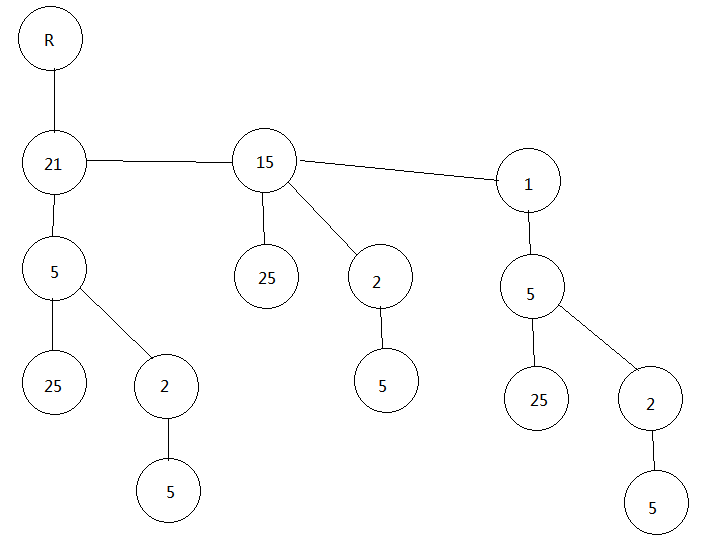
\includegraphics[width=0.6\textwidth]{tree.png}
		\end{figure}
		
		\pagebreak
		
		
		and we use this little program to list all possibilities to give us hints.
		
		\item Since the message is not very long and encoding method is easy, we just use our English knowledge to test whether the words make sense in its place.
		
	\end{enumerate}
	
	And finally, we solve this assignment and decrypt message M shown as following:\\
	
	
	1 12 12 25 15 21 7 15 20 20 15 4 15 9 19 20 18 25 20 18 25 1 12 9 20 20 12 \\
	\indent 5 20 5 14 4 5 18 14 5 19 19\\
	
	all you got to do is try try a little tenderness
	
	\pagebreak
	
	\begin{thebibliography}{99}
		
		\bibitem{contini} Scott Patrick Contini, [\textit{Factoring Integers with the Self-Initializing Quadratic Sieve}], 1997
		
		\bibitem{silverman} Robert D. Silverman, [\textit{The Multiple Polynomial Quadratic Sieve}], Mathematics of Computation, Volume 48, Issue 177(Jan., 1987), 329-339.
		
		\bibitem{bosko} LINDSEY R. BOSKO, [\textit{FACTORING LARGE NUMBERS, A GREAT WAY TO SPEND A BIRTHDAY}]
		
		\bibitem{twenty} Dan Boneh, [\textit{Twenty Years of Attacks on the RSA Cryptosystem}]
		
		\bibitem{atale} Carl Pomerance, [\textit{A Tale of Two Sieves}], December 1996
		
		\bibitem{joy} Samuel S. Wagstaff, Jr., [\textit{The Joy Of Factoring}], STUDENT MATHEMATICAL LIBRARY Volume 68, 2013, Chapter 8
		
		\bibitem{simple} Eric Landquist, [\textit{The Quadratic Sieve Factoring Algorithm}], December 14, 2001, Graduation Paper
		
		\bibitem{pomerance} Pomerance, [\textit{Smooth Numbers and the Quadratic Sieve }], Algorithmic Number theory MIRI Publication Volume 44, 2008
		
		\bibitem{williams} H.C. Williams, [\textit{A p+1 Method of Factoring}], Mathematics of computation volume 39, Number, 159 July 1982
		
		\bibitem{charest} Annie-Sophie Charest, [\textit{Pollard's p-1 and Lenstra's factoring algorithms}], Oct.2,2005
		
	\end{thebibliography}
	
	
\end{document}